\subsection{Проверка корректности загрузки данных}

\begin{itemize}	
	\item В "<1С Розница"> открываем обработку «ВыгрузитьОстаткиНаДату.epf»
	\item Указываем дату конца периода.
	\item Нажимаем \keys{Сформировать остатки}.
	Рис.~\ref{ris:9.jpg}	
	\begin{figure}[H]
		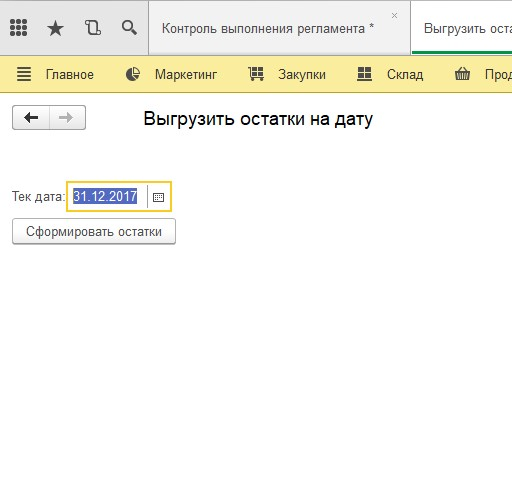
\includegraphics[width=0.5\textwidth]{9.jpg}
		\caption{Выгрузка остатков на дату.}
		\label{ris:9.jpg}
	\end{figure}
Будет сформирован файл с остатками товара "<D://Ost\_rozn.txt"> . На компьютере с "<1С Розница">	

	\item В «УТ» открываем обработку «СравнениеОстатков.epf»
	Рис.~\ref{ris:10.jpg}	
	\begin{figure}[H]
		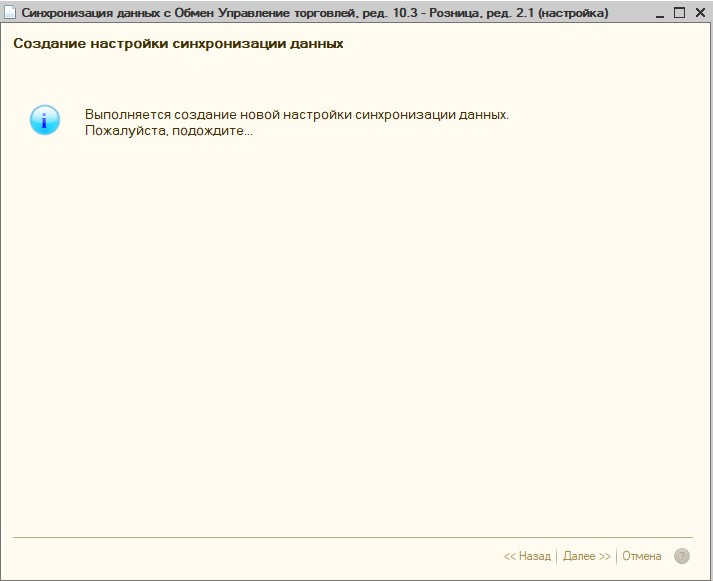
\includegraphics[width=0.6\textwidth]{10.jpg}
		\caption{Контроль остатков.}
		\label{ris:10.jpg}
	\end{figure}	
	\item Указываем дату (последний день периода) и путь к файлу с остатками.
	\item Нажимаем \keys{Сравнить}.	
	Рис.~\ref{ris:11.jpg}	
	\begin{figure}[H]
		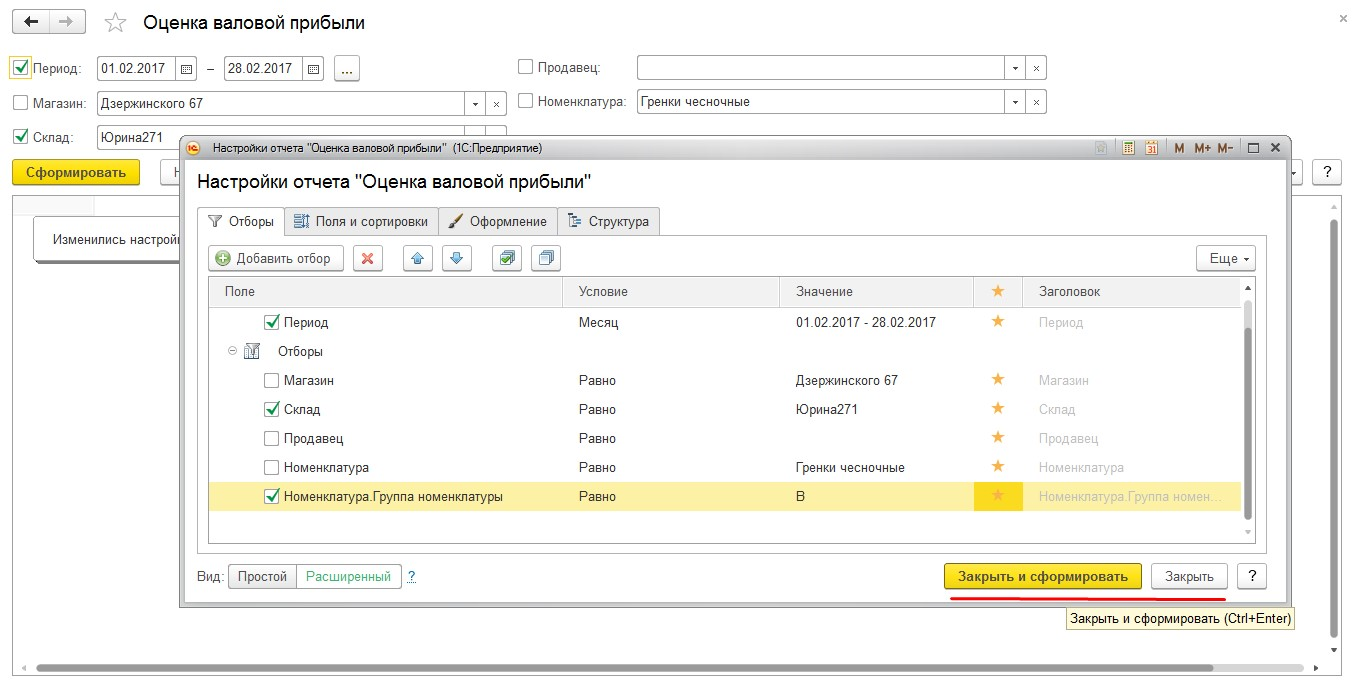
\includegraphics[width=0.6\textwidth]{11.jpg}
		\caption{Сверка остатков.}
		\label{ris:11.jpg}
	\end{figure}		
Допустимо расхождение остатков только по комплектующим кулинарии. \par


	\item Формируем в «1С Рознице» отчет «Оценка валовой прибыли» и формируем в «УТ» итоговый отчет. Сравниваем цифры валовой прибыли (должна совпадать) и себестоимости (допустимо расхождение). 


%	\item Нажимаем \keys{Загрузить данные}.
%	\item Выбираем следующий файл и повторяем процесс.
%	\subsubsection{Порядок загрузки}	
%	\item Первыми загружаем справочники. Придерживаясь порядка в дереве объектов.
%	\item Вторыми загружаем регистры сведений. Придерживаясь порядка в дереве объектов.	\sidenote[-6ex][a]{Загрузка регистра себестоимости может занять достаточно продолжительное время!}
%	\item Последними загружаем документы. Придерживаясь порядка в дереве объектов. \par \par
%	Загрузка завершена, теперь переходим к этапу проверки.\footnote{Ошибки возникающие в процессе загрузки, чаще всего связаны с необходимости корректировки правил. Так же возможны ошибки возникающие в процессе записи или проведения объекта, подобные ошибки можно проанализировать и исправить по окончанию загрузки данных}	
%	
\end{itemize}
